\section{Alert Expectations} \label{sec:alerts}


In this section we highlight issues alert users may wish to be aware of.


\subsection{Identifying Alerts with DECam Templates}

Starting in alert schema v11.2, we added several columns to the diaSource table to enable users to recognize when alerts come from difference images generated from DECam templates. 
They are:

\eric{summarize}

\subsection{Alert Rates}

\todo{summarize pilot}

\subsection{Expected Origins of Additional DiaSources}

DiaSources originate in positive and negative $5\sigma$ excesses in the difference images.
While Real/Bogus scoring \citep{DMTN-337} attempts to ensure that the resulting alerts that result are astrophysical, the classifier is ultimately morphological in nature.  
We note several cases where Rubin$-$DECam will generate more diaSources than Rubin$-$Rubin for the same science image:

\subsection{Bandpass Differences}

Sources with extreme colors may appear as diaSources due to differences in the net filter throughput.
Absent other variability, these sources will have constant difference image flux and and be filtered using timeseries features.

\todo{would be nice to make a plot or so here showing what counts as extreme}

\subsection{Stellar Proper Motion}

% Many stars will exhibit proper motions between the epoch of the DECam template and the current Rubin image.
% In difference images, these will appear as dipoles with positive and negative lobes.
% The `isDiplole` flag may be used to efficiently remove such sources, which are also typically given lower scores by Real/Bogus.
% Users interested in proper motions may make use of the dipole fit parameters and the template epoch information provided.
We find that many new dipoles detected in Rubin-DECam difference images, including those with high reliability scores, are not transients or artefacts of subtraction, but rather represent true astrophysical motion of stars. The DECam templates are built from exposures taken about a decade before the Rubin visits, so any star whose proper motion over that interval is comparable to the PSF width leaves a dipole in the difference images. We crossmatched all \texttt{diaSources} from the Rubin-DECam difference images to Gaia DR3 and selected those with a successful dipole fit and a Gaia proper motion, giving 46 dipoles. The measured dipole length, \newline $\texttt{ip\_diffim\_DipoleFit\_separation}$ (or $\texttt{dipoleLength}$ in the APDB), agrees with the expected displacement of the star, Gaia proper motion multiplied by the interval between the epoch of the DECam template and the current Rubin image ($\approx$10.62 years), in magnitude (figure \ref{fig:gaia_pms}) as well as in direction. Thus, we recommend that the users interested in extragalactic transients or variable stars to make use of the Gaia proper motion catalog to identify and remove stars that will lead to dipoles.
\begin{figure}[h]
    \centering
    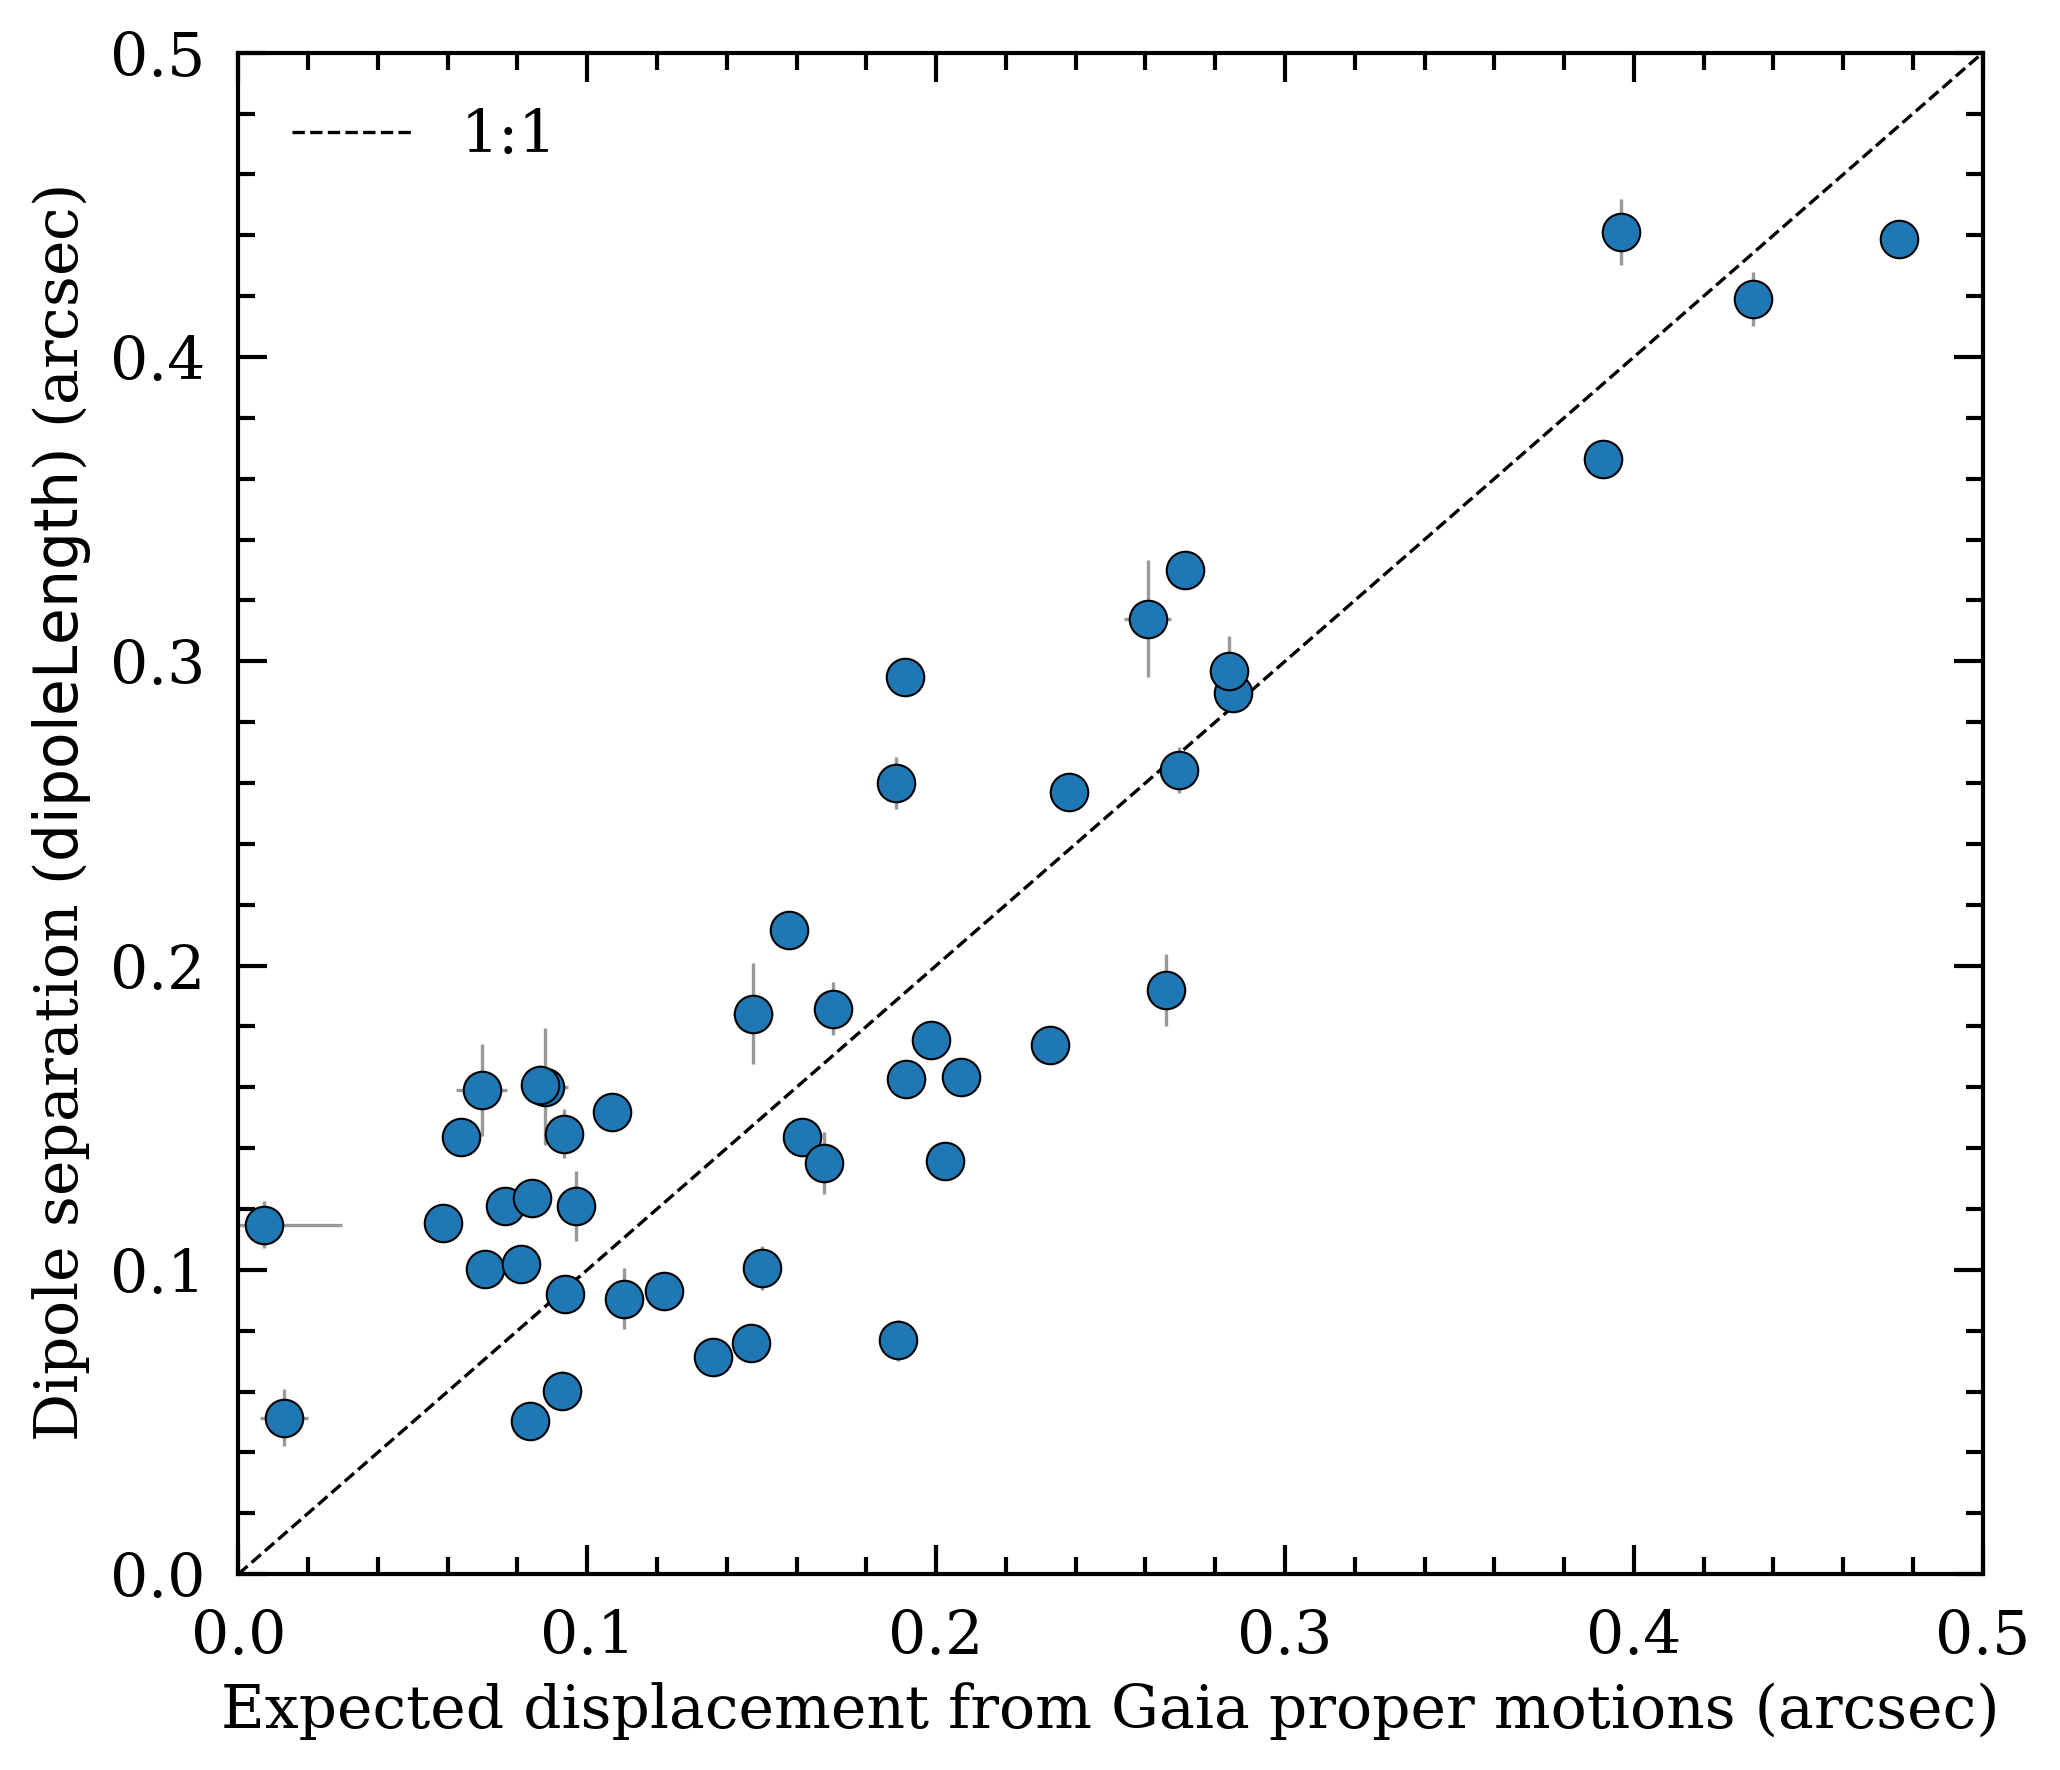
\includegraphics[width=0.65\linewidth]{figures/gaia_pms.png}
    \caption{The comparison of dipole separation measured by the pipeline dipole fit and the displacement expected from Gaia DR3 proper motion over the template-to-science interval of $\approx$10.62 years, for 46 DiaSources classified as dipoles and matched to Gaia stars with measured proper motions from one CCD difference image. The error bars show the errors on the proper motions and dipole separations obtained via error propagation from the errors on their individual components.
    }
    \label{fig:gaia_pms}
\end{figure}

\subsection{Long-term Variability}

Given the longer temporal baseline, slow-varying sources such as AGN are more likely to appear as significant difference image sources with DECam templates.
This corresponds to real astrophysical variation.

\subsection{Other Artifacts and Mismatches}




\subsection{Real-Bogus Performance}